%--------------------------------------------------------------------
% \chapter{Sensor Collection Service}
%--------------------------------------------------------------------
\label{chap:SensorCollection}

\section{Mobile Sensor Collector}
\label{sec:SensorColllection}

In this deliverable we present the a revised sensor collection
component. It offers the following improvements over the last version
presented in D1.1:
\begin{itemize}
\item High performance recordings on Low-End devices. During the field
  trial some low-end devices showed difficulties to record the sensor
  samples with sufficient frequency. We streamlined the architecture
  in order to reduced the overhead caused by the processing of the
  samples. For example, we traded the convenience of a SQL database in
  favor of the performance benefits of a flat file solution.  Also, in
  this process we removed dependency on external SDCF
  library\footnote{\url{http://www.sdcf.eu/}}, and reimplemented core
  parts of the component.
\item Improved battery awareness. Power consumption in the sensor
  collection process is largely driven the GPS sensor. In May 2013
  Google released a new location API, that takes advantage of multiple
  location provider and reduces the power consumption significantly.
  The revised component makes use of this new API, and offers a
  fallback in case the service is not supported by the device.
\item Revised export format. We have improved the data exchange
  formats used for publishing samples to other components and storage
  on the central server. In section \ref{sec:ssf} we specify the
  ssf-Sensor Stream Format, which is inspired by the
  \href{http://en.wikipedia.org/wiki/Common\_Log\_Format}{Common Log
    Format} used by many webservers. It allows easy human inspection
  and processing by standard (UNIX) tools like ``grep'' and ``sed''
  while being reasonably memory efficient.
\item Streaming API. The streaming API is a new communication channel
  between the mobile sensor collector and the central server. It
  allows to transfer the incoming sensor data directly to the server
  using the ssf format.
\item Integration into Live+Gov Service Center. The revised sensor
  collector and sensor storage service is compatible with the Live+Gov
  service center. This feature allows central user management as well
  as health monitoring and centralized log aggregation of the services.
\item Seamless Extendability. The revised architecture can be easily
  extended by further stream processing components. This is realized
  by a dispatcher thread that distributes sensor samples to registered
  components over a simple interface (again using ssf). Implemented
  extensions include the Human Activity Recognition component
  (c.f. section \ref{sec:HAR}) and a GPS-sample publisher component
  that is used by the Service Line Detection service (cf. section
  \ref{sec:SLD}).
\end{itemize}

\subsection{Architecture Description}

The new architecture is sketched in Figure \ref{fig:sc_architecture}.
It consists of the following components:

\begin{figure}[h]
\centering
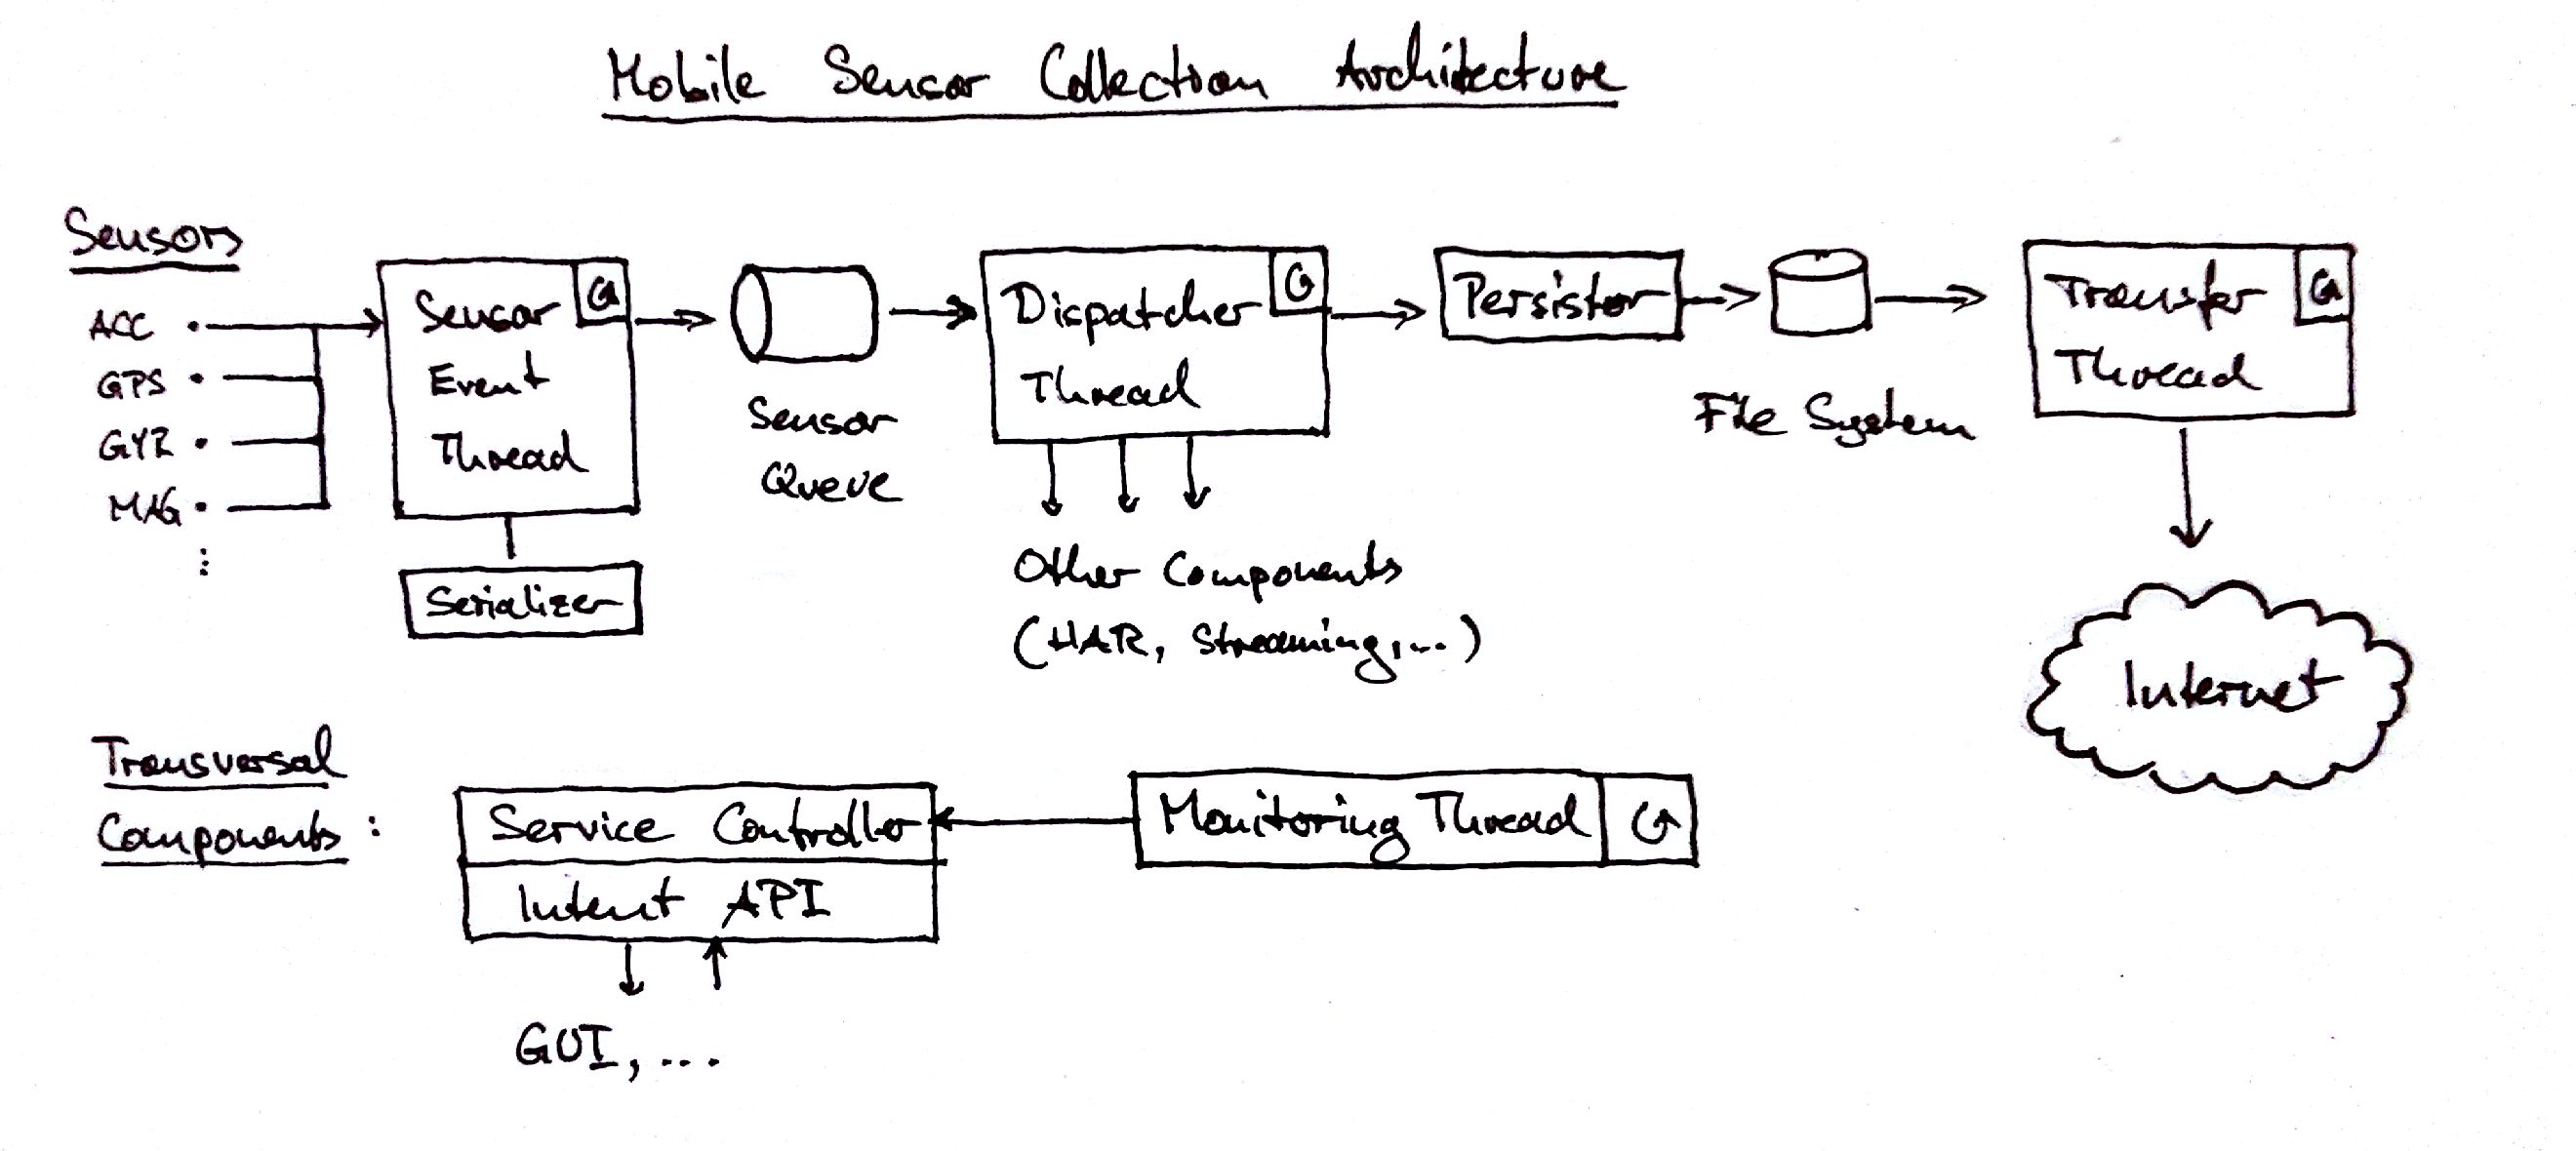
\includegraphics[width=\textwidth]{img/sc/sc_architecture.jpg}
\caption{Sensor Collection Architecture}\label{fig:sc_architecture}
\end{figure}

\begin{itemize}
\item {\bf Sensor Event Thread}. The sensor event thread registers
  callback listeners for all configured sensors. When sensor events
  occur the received values are serialized in the ssf
  format (cf. \ref{sec:ssf}) and pushed onto the SensorQueue.
\item {\bf SensorQueue}. The sensor queue is a synchronized queue
  object that stores sensor values as strings.
\item {\bf DispatcherThread}. The dispatcher thread reads sensor
  values from the sensor queue and passes them to several services
  that can be registered. Included services are the persistor service
  and the activity recognition component, the streaming service and GPS
  publication pipeline (for use in the Service Line Detection API).
\item {\bf Persistor}. The persistor service is executed by the
  DispatcherThread and appends the received sensor sample into a
  predefined file. Also a variant with zip-file compression is
  included.
\item {\bf TransferThread}. The transfer thread is an independent
  thread that transfers the persisted samples to the Live+Gov servers.
\item {\bf Monitoring Thread}. The monitoring thread polls the
  different components and gathers run-time information like numbers
  of processed samples or transfer state.
\item {\bf Service Controller}. The service controller starts and
  stops all threads, and takes care of proper configuration of all
  services. It listens to intents specified in the API and changes the
  state of the service accordingly.
\end{itemize}

The supported sensors are summarized in Table
\ref{fig:sensor_table}. They are unchanged from D1.1.

\begin{figure}
\centering
\begin{tabular}{|l|p{0.7\linewidth}|}
  \hline
  Sensor & Description \\
  \hline
  GPS                 & Global position in latitude and longitude. 

                        If available, the GPS samples are gathered via
                        Google's new Play Services location
                        provider\footnote{https://developer.android.com/google/play-services/location.html}.
                        
                        If the Play Services are not available, the service falls back to
                        accessing the GPS samples directly.
  \\ \hline
  Accelerometer       & Measures the acceleration force in $m/s^2$
                        that is applied to a device on all three
                        physical axes. 

                        Also the low-pass and high-pass filtered
                        variants 'Linear Acceleration' and 'Gravity' offered by the Google
                        API can be captured.
  \\ 
  Rotation Vector     & Measures the orientation of a device by
                        providing the three elements of the device's
                        rotation vector.  
  \\
  Gyroscope           & Measures a device's rate of rotation in
                        $rad/s$ around each of the three physical
                        axes. 
  \\ 
  Magnetic field      & Measures the ambient geomagnetic field for all
                        three physical axes in $\mu T$. 
  \\ \hline
  WLAN                & A list of all available wireless local area
                        networks in the transmission range. 
  \\
  Bluetooth           & A list of all available bluetooth clients in
                        the transmission range. 
  \\
  GSM                 & Cellular network operator and the radio cell
                        the mobile phone is connected with. 
  \\ \hline
  Google Activity     & Google recently released an Activity
                        Recognition Library. The sensor collector is able to record activities as sensor
                        values as well. 
  \\
  \hline
\end{tabular}
\caption{Supported sensors of the Sensor Collector}
\label{fig:sensor_table}
\end{figure}

\subsection{Intent API}
\label{subsubsec:IntentAPIdescription}

The communication with other Live+Gov toolkit components is
facilitated through the exchange intent
messages\footnote{\url{http://developer.android.com/guide/components/intents-filters.html}}.
The API was slightly improved since deliverable D1.1. We removed the
explicit ``Start/Stop Service'' intents, since the service now shuts
down automatically when no services are requested. The following list
summarizes all provided intent controls. New intents are marked with
an asterisk (*).

\begin{itemize}
\item {\bfseries Start/Stop Recording.} Starts and stops recording of
  sensor samples. Samples are persisted in a local sensor file.
\item {\bfseries Delete Samples.*} Delete all stored samples on the
  device.
\item {\bf Send Annotation.} This intent allows users to annotate
  their recording by a string value that will be recorded by a
  ``tag-sensor''.
\item {\bfseries Enable/Disable Streaming*.} When enabled, all
  collected sensor samples are streamed over to a central server over
  the network. See section \ref{sec:straming} for more details.
\item {\bfseries Transfer samples.}  Controls the sample transfer
  state machine. When enabled and a network connection is available
  sensor samples are transferred in batches to the server backend.
\item {\bfseries Enable/Disable sample broadcast.} When enabled all
  recorded sensor samples are broadcasted in the form of intents into
  the system. This allows other components, e.g. feature extraction
  and context mining, to make use of the recorded sensor data.
\item {\bfseries Request Status Report.} When this intent is received
  a status report is broadcasted to the system. A summary of returned
  information is shown in Figure \ref{tab:StatusIntent}.
\item {\bfseries Set user ID.*} Set the user id to a given value. This
  intent is used to connect the mining results to the user data in the
  Live+Gov service center.
\item {\bfseries Get GPS samples.*} Returns a summary of the latest
  GPS samples gathered by the system in ssf format. It is intended to
  be used by the service line detection service described in Section \ref{sec:SLD}.
\end{itemize}

When a control intent is received by the component, the appropriate
action is taken. After execution has finished a status report intent
is broadcasted to the system which provides information about whether
the requested method call was successful. Further technical
description of the component and the API are included in D4.1.

\begin{figure}[ht]
\centering
\begin{tabular}{|l|l|l|} \hline
   Key       & Type    & Description                                       \\ \hline
   running   & boolean & True if service is running.                       \\
   recording & boolean & True if sensor samples are recorded.              \\
   storage   & boolean & True if samples are stored in the database.       \\
   transfer  & boolean & True if continues transfer of samples is enabled. \\
   broadcast & boolean & True if samples are broadcasted.                  \\ \hline
\end{tabular}
\caption{Structure of status intents}
\label{tab:StatusIntent}
\end{figure}

\subsection*{Component Testing}

The sensor collector comes accompanied with a testing GUI shown in
Figure \ref{fig:sc_gui}, that provides buttons for the implemented
intent controls API. The returned status information is displayed in
the form of plain text logs, button states and spinners.

The GUI can be used to test the functionality of the component and for
the gathering of training data.

In addition we provide automated unit-test cases for the intent API
along with the source code.


\begin{figure}[h]
\centering
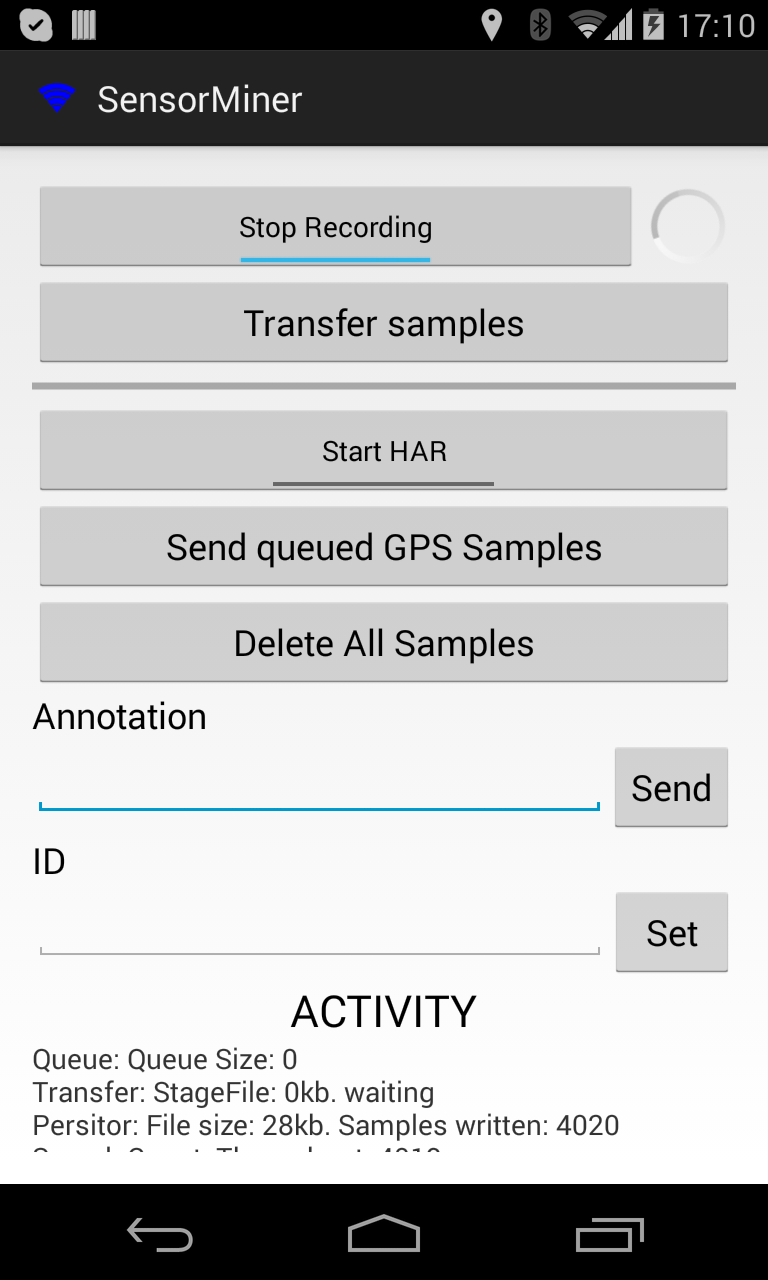
\includegraphics[width=0.3 \textwidth]{img/sc/sc_gui.png}
\caption{Sensor Collection Architecture}\label{fig:sc_gui}
\end{figure}

\subsection{Sensor Stream Format (ssf)}\label{sec:ssf}
The sensor stream format ({\it ssf}) which is used for transfering
sensor values from a mobile device (or another sensor source) to the
Live+Gov data-base. The file format is inspired by the
\href{http://en.wikipedia.org/wiki/Common\_Log\_Format}{Common Log
  Format} used by many webservers. It replaces the XML-based format
used in D1.1. We view incoming sensor values as events and record them
as a simple stream of CSV-rows. Each sensor has an individual prefix
but writes into the same file.

The key advantages of this format as opposed to the previously used
XML format are:
\begin{itemize}
\item Human readability. The format is easy to understand by humans.
\item Flexibility. Every line can be interpreted without the context
  of the file. Therefore ssf-files can be arbitrarily sliced,
  concatenated and filtered using UNIX tools like {\it grep, cat, sed,
    awk}.
\item Streaming support. Lines can be individually transferred over tcp
  sockets or messaging systems. Allowing immediate inspection of the
  recorded samples on a remote system.
\end{itemize}

The rows of the ssf-format have the following structure:
\small
\begin{verbatim}
SENSOR_PREFIX,TIME_STAMP, USER_ID, SENSOR_VALUES
\end{verbatim}
\normalsize

\begin{itemize}
\item \texttt{SENSOR PREFIX}. Identifies the sensor producing the
  sample. The following sensor prefixes are supported: \\
  \texttt{GPS} (GPS sensor), \texttt{ACC} (Accelerometer),
  \texttt{LAC} (Linear Acceleration), \texttt{GRA} (Gravity),
  \texttt{GYR} (Gyroscope), \texttt{MAG} (Magnetometer), \texttt{WIFI}
  (Wifi networks), \texttt{BLT} (Bluetooth), \texttt{GSM} (GSM cells),
  \texttt{ACT} (Google Play Services Activity), \texttt{ERR} (Error
  Value), \texttt{TAG} (Annotations entered by the user).
\item \texttt{TIME STAMP} UNIX timestamp in milliseconds
  e.g. \texttt{1377609577214}
\item \texttt{USER ID} ID that identifies records from the same
  user. The default value is the device-id that is provided by
  Android.
\item \texttt{SENSOR VALUES} Sensor values in individual formats. In
  order to adhere to the CSV standard no \texttt{,}-symbol and
  new-lines may be used in this field.
  \begin{itemize}
  \item \texttt{ACC/GYR/MAG/LAC/GRA} x,y,z-values separated by space characters.
  \item \texttt{GPS} lat,lon,alt-values separated by space characters
  \item \texttt{ACT} Activity Name, Confidence separated by space characters.
  \item \texttt{WIFI} List of access-points, where each visible
    accesspoint is separated by a \texttt{;} and written as \\
    {\it Escaped SSID String/Escaped BSSID String/Frequency in MHz/RSSI in dBm}
  \item \texttt{BLT}
    List of devices where each visible device is separated by a \texttt{;}
    and written as \\
    { \it Escaped Address/Device Major Class/Device Class/Bond
      State/Optional Escaped Name/Optional RSSI }
  \item \texttt{GSM}
    The state of the device written as Service State/Roaming State/Manual
    Carrier Selection State/Escaped Carrier Name/Escaped Signal Strength
    followed by \texttt{:}, followed by a possibly empty list of cells,
    where each cell is separated by a \texttt{;} and written as: \\
    {\it Escaped Cell Identity/Cell Type/RSSI in dBm}
  \end{itemize}
\end{itemize}

Example rows may look as follows:
\small
\begin{verbatim}
ACC,1377605748123,5,0.9813749 0.0021324 0.0142523
GPS,1377605748156,5,50.32124 25.2453 136.5335
WIFI,1341244415,wifiUser,"WiFi AP"/"00:12:42"/2412/-45; \\
                  "Another WiFi AP"/"33:13:53"/2437/-56
TAG,1378114981049,anotherUser,"test tag"
BLT,1385988380374,bluetoothUser,"C8:F7:33:B7:B5:B4" \\
                  /computer/computer laptop/bonded/"LAPTOP"/-46
\end{verbatim}
\normalsize

\subsection{Streaming Service}\label{sec:straming}

The revised version of the sensor collector includes a streaming
service, that transfers recorded samples directly to a remote machine.
The streaming service uses the ZeroMQ networking
library\footnote{http://www.zeromq.org} to transfer single ssf lines
to the Live+Gov machine running a streaming server. The streaming
server appends the received samples to a file (zmq\_stream.ssf).

This simple service allows direct monitoring of the recorded samples,
via simple UNIX command line tools. 
\begin{itemize}
\item \texttt{tail -f zmq\_stream.ssf} - prints the recoded samples to the console.
\item \texttt{tail -f zmq\_stream.ssf | grep GPS} - filters out GPS samples.
\item \texttt{tail -f zmq\_stream.ssf | cut --delimiter=',' --field=1 | logtop}\\
  shows the frequencies of the individual incoming sensor values.
\end{itemize}

\section{Sensor Storage Service}

The sensor storage service runs on the Live+Gov servers and stores the
sensor samples collected by the mobile sensor collection component.
The storage component offers a HTTP/REST interface to upload sensor
data.  The uploaded samples are stored in a
PostgreSQL\footnote{http://www.postgresql.org/} database with
PostGIS\footnote{http://postgis.net/} plugin for Geo queries.

The architecture is sketched in \ref{fig:ss_architecture}. It consists
of the following components.
\begin{itemize}
\item {\bf Request Handler.} Java/Tomcat Servlet that provides the
  HTTP interface for sample upload. The received samples are stored in
  the file system for backup in order to have a backup and passed to
  the DB ingester thread. When both operations where successful a
  response code "202 Accepted" is sent back to the client.
\item {\bf DB Ingester.} Stores sensor samples in a database. 
  The samples are provided in ssf format and written to a PostgreSQL
  database with schema described in Figure \ref{fig:db_scheme}.
\item {\bf Inspection tool.} This component allows to inspect the
  stored samples in the database in a convenient way and prepare and
  export them for usage in the data mining task. Figure
  \ref{fig:inspection} shows a screenshot of two views of the front
  end. We are currently expanding this tool to also include
  visualizations of the data mining results.
\end{itemize}

For integration with the Live+Gov service center, we provide an
external service, that probes the upload URL in regular intervals and
sends health checks and uploads log files to the central server as
described in deliverable D4.2.

\begin{figure}
\centering
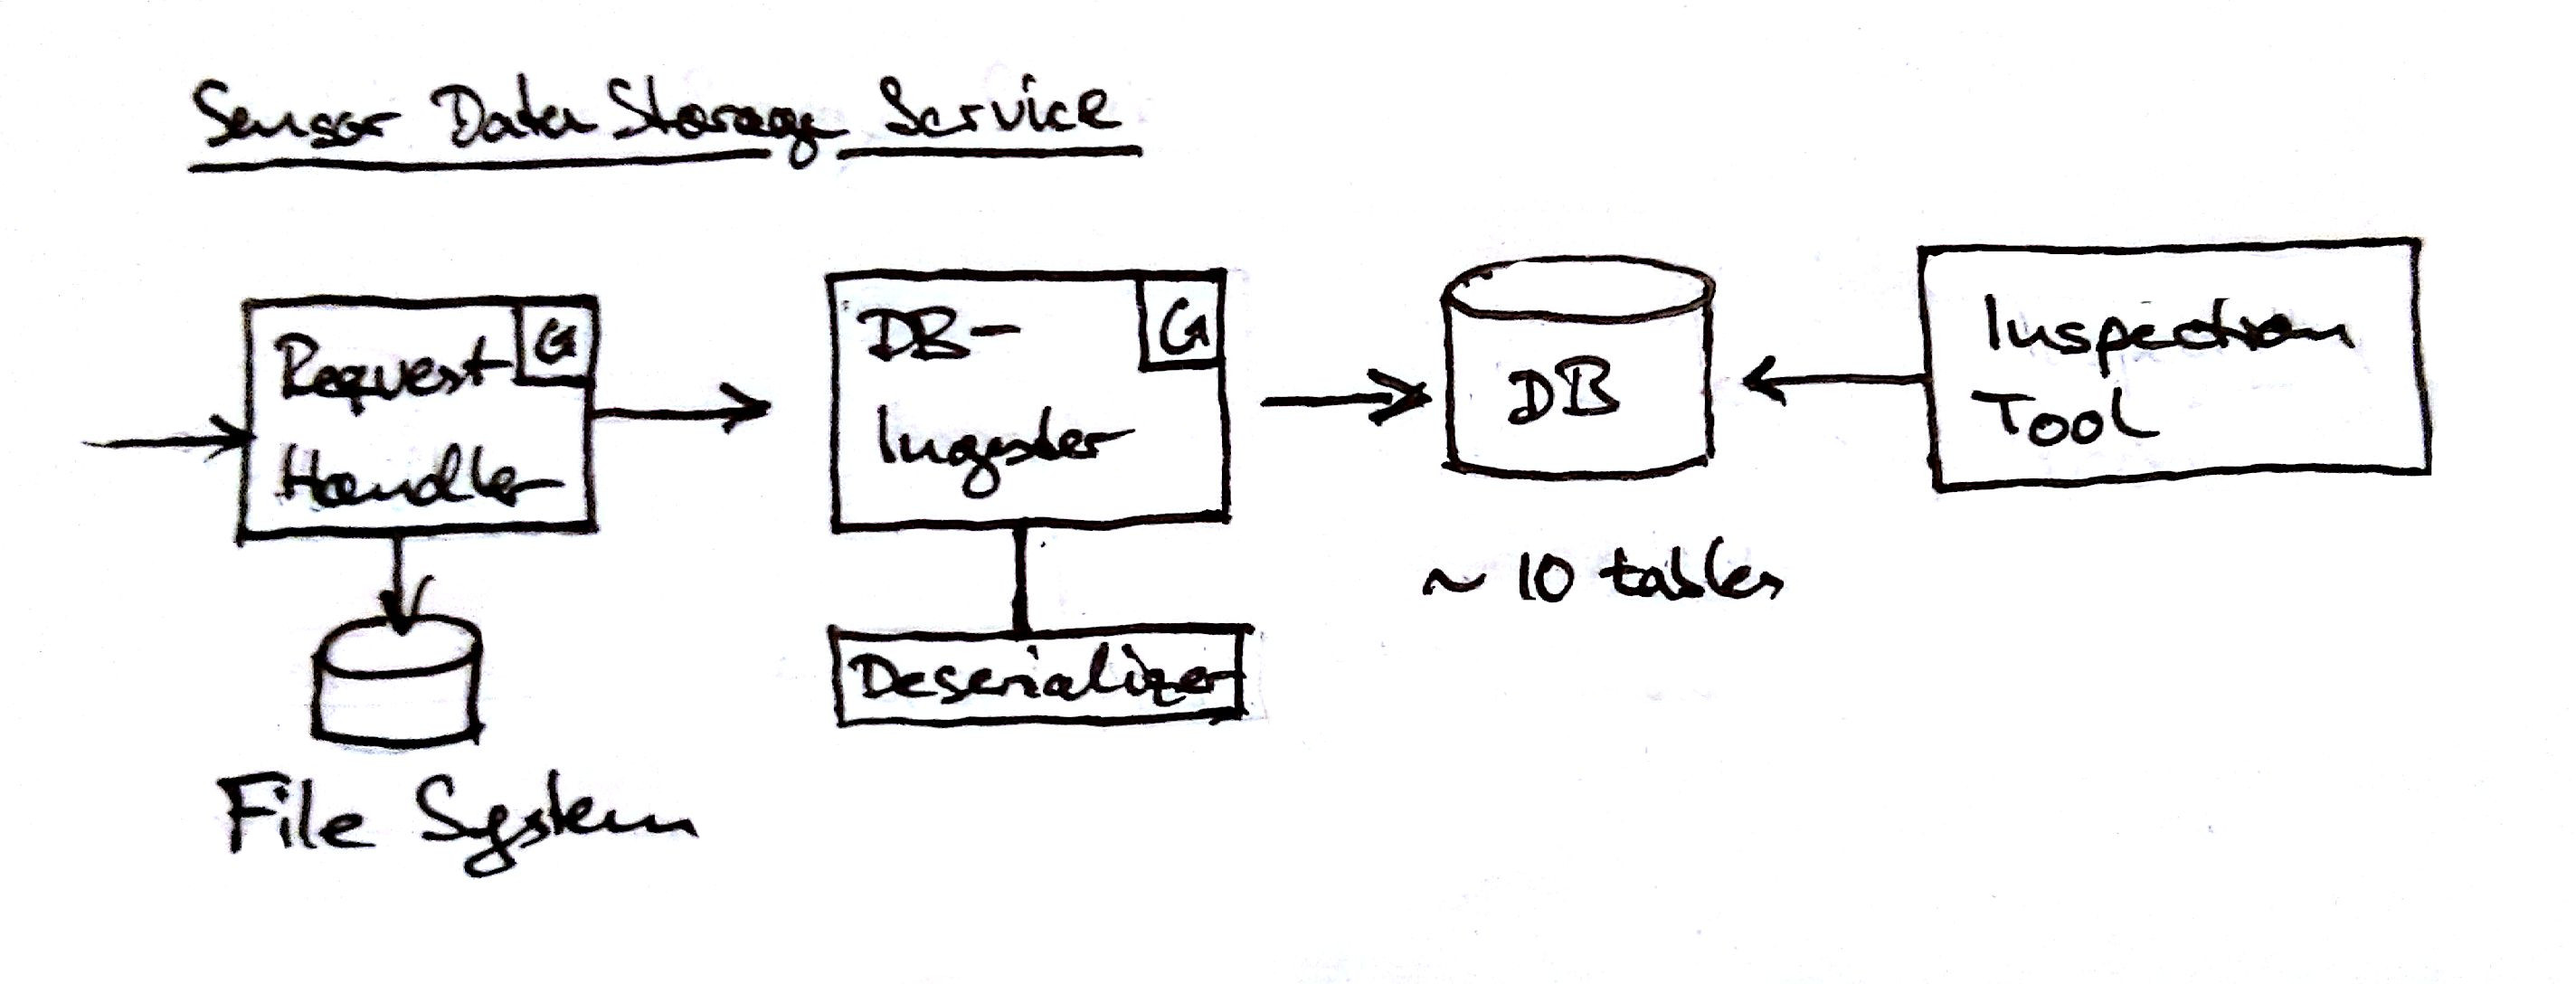
\includegraphics[width=0.7\textwidth]{img/sc/ss_architecture.jpg}
\caption{Sensor Collection Architecture}\label{fig:ss_architecture}
\end{figure}

\begin{figure}
{\small
\begin{verbatim}
sensor_gps (trip_id INT, ts BIGINT, lonlat GEOGRAPHY(Point));
sensor_accelerometer (trip_id INT, ts BIGINT, 
     x FLOAT, y FLOAT, z FLOAT);
sensor_linear_acceleration (trip_id INT, ts BIGINT,
     x FLOAT, y FLOAT, z FLOAT);
sensor_gravity (trip_id INT, ts BIGINT, 
     x FLOAT, y FLOAT, z FLOAT);
sensor_tags (trip_id INT, ts BIGINT, tag TEXT);
sensor_google_activity (trip_id INT, ts BIGINT, activity TEXT);
har_annotation (trip_id INT, ts BIGINT, tag TEXT);
\end{verbatim}}
\label{fig:db_scheme}
\caption{Schema of the Sensor Storage DB}
\end{figure}

\begin{figure}[ht]
  \begin{minipage}[b]{0.45\linewidth}
    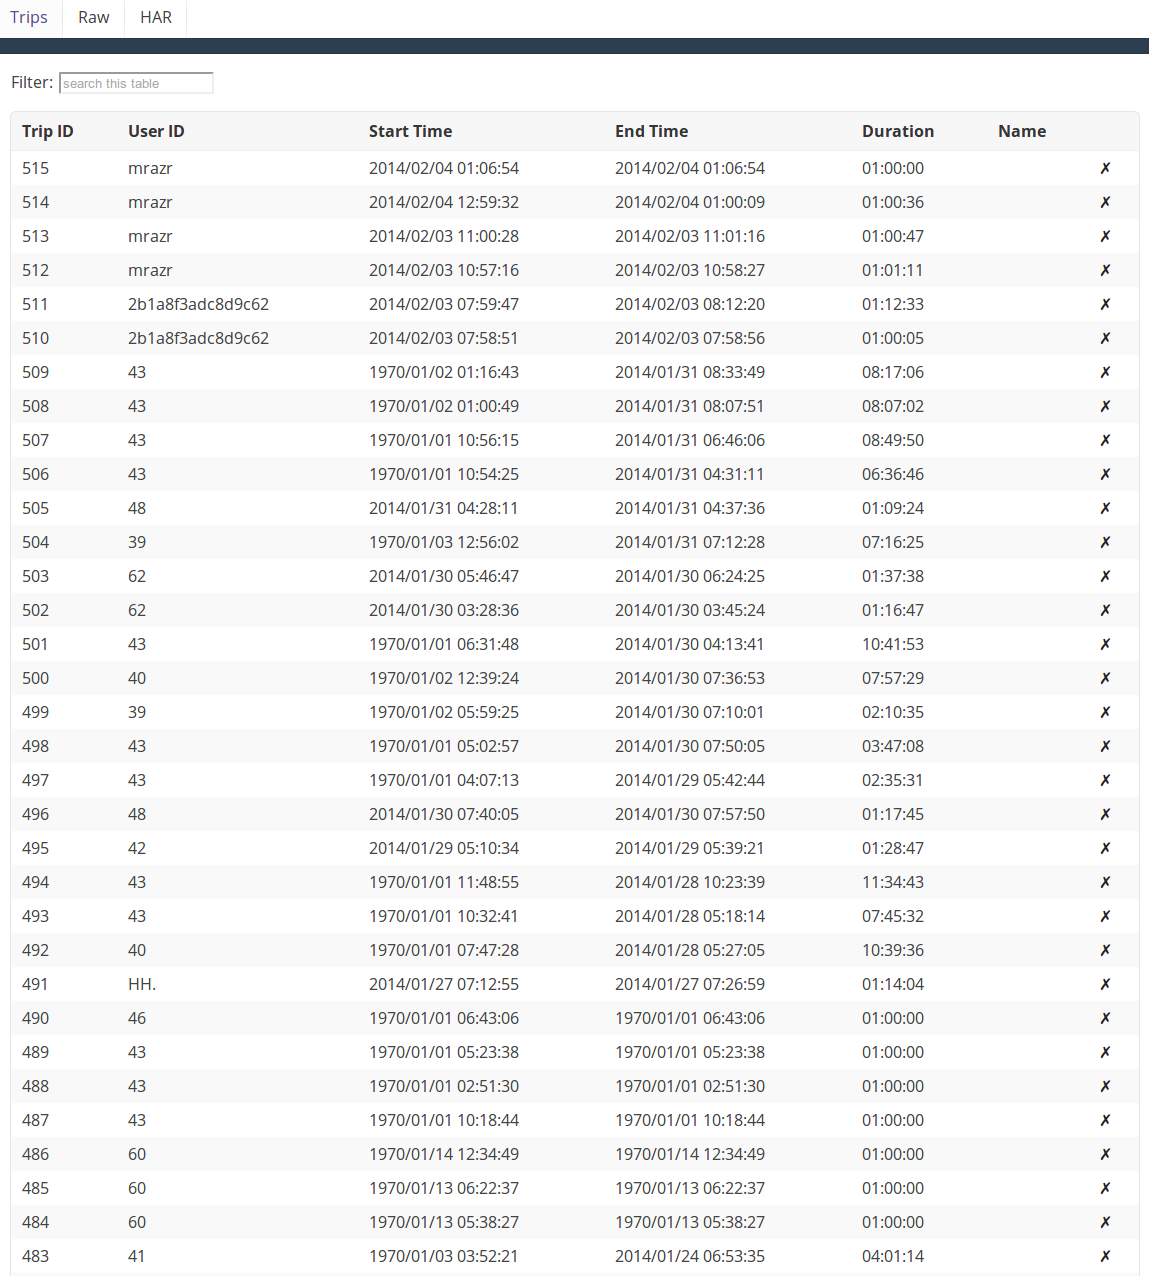
\includegraphics[width=0.9 \textwidth]{img/sc/inspection_table.png}
    \caption{Meta table}\label{fig:minipage1}
  \end{minipage}\quad
  \begin{minipage}[b]{0.45\linewidth}
    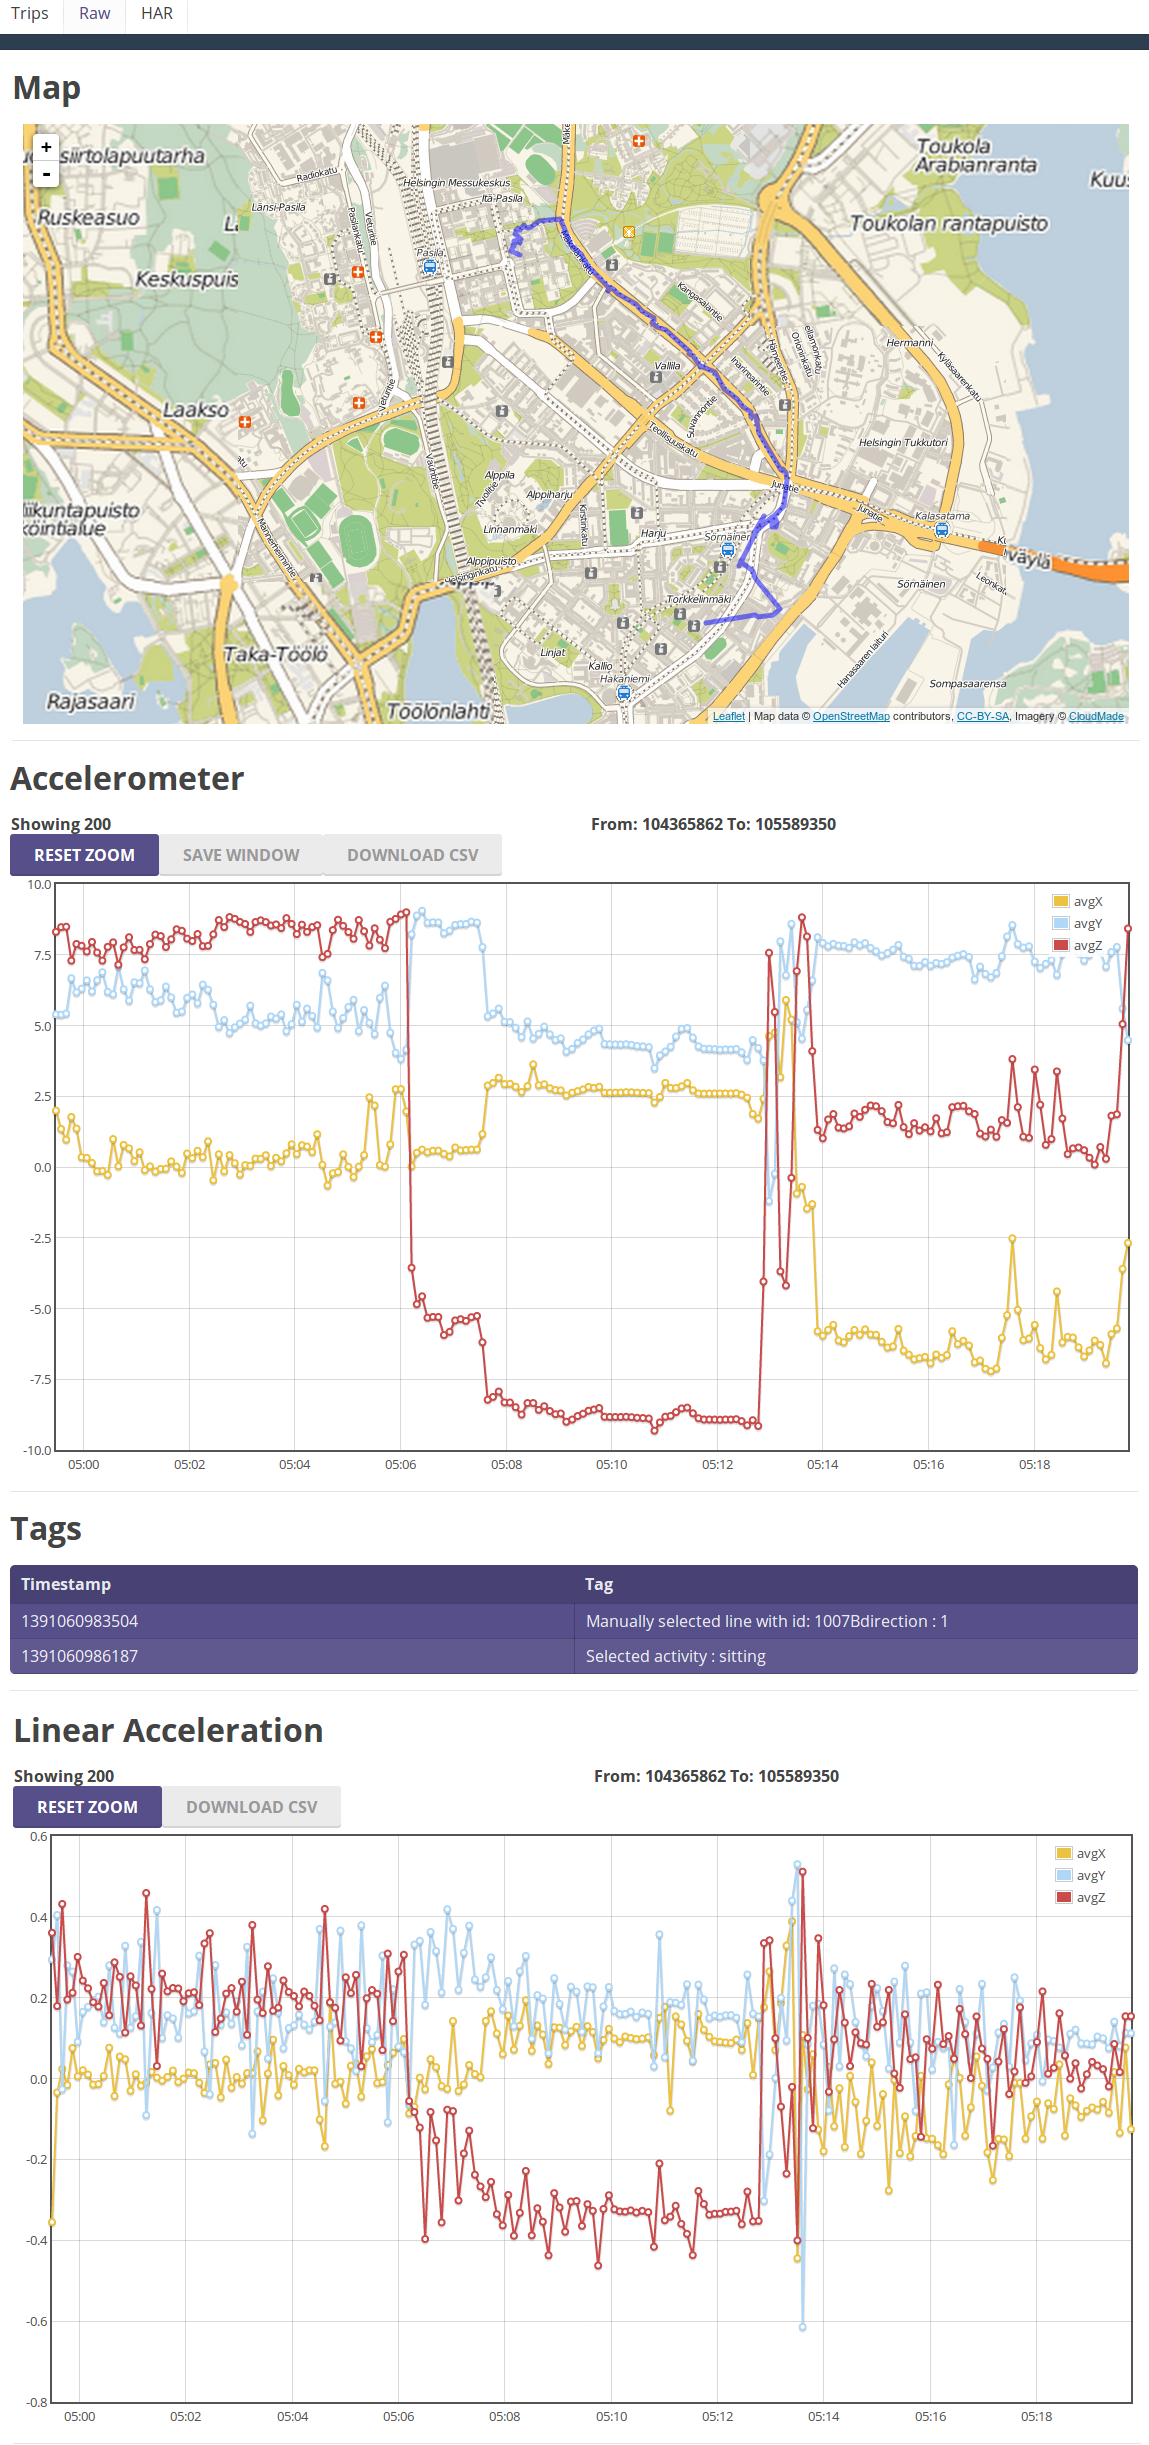
\includegraphics[width=0.9 \textwidth]{img/sc/inspection_raw_tab.png} 
    \caption{Raw data inspection view}\label{fig:minipage2}
  \end{minipage}
  \caption{Inspection Web Tool}
  \label{fig:inspection}
\end{figure}

%%% Local Variables:
%%% mode: latex
%%% TeX-master: "../D1-2"
%%% End:
